\subsection{Azimuthale äquidistante Projektion}
\label{sec:azimuequi}
Bei dieser Projektion ist die kürzeste Entfernung vom Mittelpunkt der Karte zu einem beliebigen anderen Punkt eine gerade Linie. Das bedeutet, dass alle Punkte, die auf einem Kreis um den Kartenmittelpunkt liegen, äquidistant sind.\\
Nachteil:\newline
Die Gebiete die auf der anderen Seite der Welt liegen, werden sehr verzehrt dargestellt. Daher ist diese Projektion für Weltkarten 
eher ungeeignet.\\
\begin{figure}[hbtp]
\centering
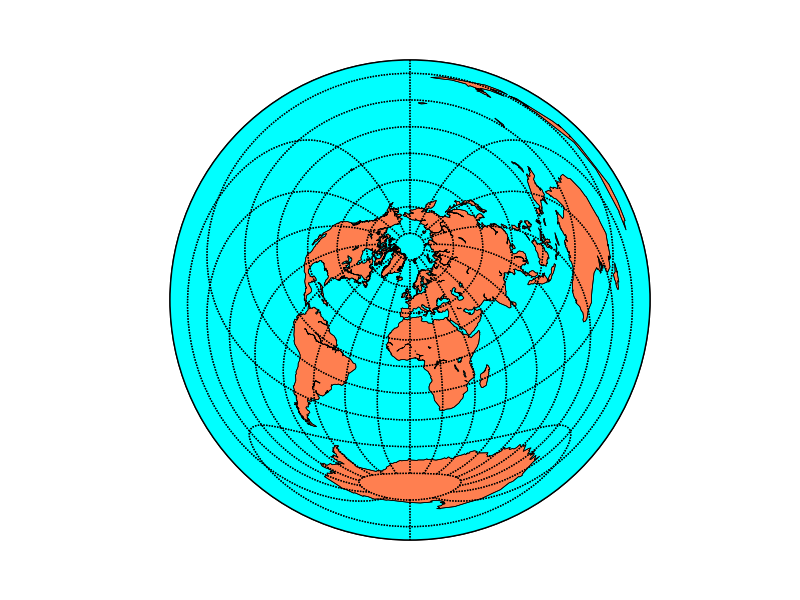
\includegraphics[scale=0.4,origin=c]{/Users/student/seminar/Kartendarstellungen/seminar/aziequi} \\
\caption{Azimuthale äquidistante Projektion}
\end{figure}
\clearpage